\documentclass[11pt]{article}
\pagestyle{empty}
\usepackage{color}
\usepackage{fancyhdr}
\usepackage{lastpage}
\usepackage[options]{algorithm2e}
\usepackage{forest}
\usepackage{tikz}
\usepackage{graphicx}
\graphicspath{ {images/} }
\tikzset{el style/.style={midway, font=\scriptsize, inner sep=+1pt, auto=right}}
\pagestyle{fancy}
\renewcommand{\headrulewidth}{0pt}
\cfoot[R]{\thepage~of~\pageref{LastPage}}
\addtolength{\oddsidemargin}{-.875in}
\addtolength{\evensidemargin}{-.875in}
\addtolength{\textwidth}{1.75in}
\addtolength{\topmargin}{-.875in}
\addtolength{\textheight}{1.75in}

\begin{document}
\begin{center} {\Large\bf FA, Homework 9} \\ Quentin McGaw (qm301) \\ 04/13/17
\end{center}

\begin{quote}
For every complex problem there is a simple solution.  And it's always wrong.
\\ H.L. Mencken, 1880-1956, American satirist.
\end{quote}

\begin{enumerate}
\item \textbf{\textcolor{blue}{(*) Suppose that the Huffman Code for $\{v,w,x,y,z\}$ has $0$ or $1$ as the code word for $z$.  {\em Prove} that the frequency for $z$ cannot be less than $\frac{1}{3}$.  {\em Give an example} where the frequency for $z$ is $0.36$ and $z$ does get code word $0$ or $1$.}}
    \\ \textbf{Proof that $z$'s frequency must be higher than $\frac{1}{3}$}
    \\ For the set $S = \{v,w,x,y,x\}$, there are 4 merges.
    \\ For $z$ to have a single bit code word with $S$, z can only be involved in the two last merges.
    Therefore there must be two first merges resulting in $m_1$ and $m_2$.
    We then have $m_1$, $m_2$ and $z$, that sum to $1.00$ and that are all $< 1.00$.
    \\ If $z$ has a frequency lower than $\frac{1}{3}$, it can't have the biggest frequency and would therefore have a two bit code word.
    \\ Therefore $z$ must have a frequency higher than $\frac{1}{3}$.
\item
\begin{enumerate}
    \item \textbf{\textcolor{blue}{What is an optimal Huffman code for the following code when the frequencies are the first eight Fibonacci number? \[ a:1, b:1, c:2, d:3, e:5, f:8, g:13, h:21  \]}}
        \\ We have the following Huffman tree: \\
        \begin{forest}
          for tree={parent anchor=south},
          where n children={0}{tier=word}{
            if={n==1}{% n == 1 means first child
              edge label={node[el style]{0}}
            }{
              edge label={node[el style, swap]{1}}
            }
          }
        %
        [54 
            [21 [h]]
            [33
                [13 [g]]
                [20
                    [8 [f]]
                    [12
                        [5 [e]]
                        [7
                            [3 [d]]
                            [4
                                [2 [c]]
                                [2
                                    [1 [b]]
                                    [1 [a]]
                                ]
                                
                            ]
                            
                        ]
                        
                    ]
                    
                ]
                
            ]
            
        ]
        \end{forest}
        \\ Hence we have $C(h) = 0$, $C(g) = 10$, $C(f) = 110$, $C(e) = 1110$, $C(d) = 11110$, $C(c) = 111110$, $C(b) = 1111110$ and  $C(a) = 1111111$. Note that the codes of $a$ and $b$ can be exchanged. Also, we obtain different codes if $0$'s and $1$'s are switched around.
    \item \textbf{\textcolor{blue}{The Fibonacci sequence is defined by initial values $0,1$ with each further term the sum of the previous two terms.  Generalize the previous answer to find the optimal code when there are $n$ letters with frequencies the first $n$ (excluding the $0$) Fibonacci numbers.}}
        \\ The encoding for the character with the first Fibonacci number is $h_1 = 1^{n-1}$.
        \\ The encoding for the character with the $i^th$ Fibonacci number is $h_i = 1^{n-k}\ 0$.
\end{enumerate}

\item \textbf{\textcolor{blue}{Suppose that in implementing the Huffman code we weren't so clever as to use Min-Heaps. Rather, at each step we found the two letters of minimal frequency and replaced them by a new letter with frequency their sum. How long would that algorithm take, in Thetaland, as a function of the initial number of letters $n$.}}
    \begin{itemize}
        \item To find the two letters of minimal frequency, we need $O(n)$ time. Adding them etc. is included in $O(n)$.
        \item As we progress, the number of letters decreases but the first $\frac{n}{2}$ times, there are at least $\frac{n}{2}$ letters and finding the minimum takes $\Omega(n)$. The total time for the first $\frac{n}{2}$ times is thus $\Omega(\frac{n}{2} \times \frac{n}{2}) = \Omega(n^2)$.
        \item From the lower and upper bounds, this gives a total time of $\Theta(n^2)$.
    \end{itemize}
    
\item \textbf{\textcolor{blue}{Consider the undirected graph with vertices $1,2,3,4,5$ and adjacency lists (arrows omitted) $1:25$, $2:1534$, $3:24$, $4:253$, $5:412$.  Show the $d$ and
$\pi$ values that result from running BFS, using $3$ as a source.  Nice picture, please!}}
    \\ Breadth first search (BFS) starts at the root of a tree and explores the neighbor nodes first, before moving to the next level neighbors.
    \\
    \begin{algorithm}[H]
    \SetKwFunction{bfs}{BFS}
    \Indm\bfs{G, s}\\
    \Indp
        \For{each vertex $u \in G.V - \{s\}$}{
            color[u] = WHITE \\
            d[u] = $\infty$ \\
            $\pi$[u] = NIL \\
        }
        color[s] = GRAY \\
        d[s] = 0 \\
        $\pi$[s] = NIL \\
        Q = $\emptyset$ \\
        ENQUEUE(Q, s) \\
        \While{Q $\neq \emptyset$}{
            u = DEQUEUE(Q) \\
            \For{each v $\in$ G.Adj[u]}{
                \If{color[v] == WHITE}{
                    color[v] = GRAY \\
                    d[v] = d[u] + 1 \\
                    $\pi$[v] = u \\
                    ENQUEUE(Q, v) \\
                }
            }
            color[u] = BLACK \\
        }
    \caption{BFS algorithm}
    \end{algorithm}
    \\ At the beginning, we start from 3 as source $s$. We set d[3] = 0 and $\pi$[s] = NIL (no parent) and add this vertex to Q so Q = $\{3\}$. \\
    \begin{tikzpicture}[auto, node distance=2cm,thick,vertex/.style={circle,draw}]
    \node[vertex] (1) [fill=white, text=black] {1};
    \node[vertex] (2) [fill=white, text=black, below left of=1] {2};
    \node[vertex] (3) [fill=gray, text=black, below right of=2] {3};
    \node[vertex] (4) [fill=white, text=black, right of=3] {4};
    \node[vertex] (5) [fill=white, text=black, right of=1] {5};
    \path
    (1) edge node {} (2)
        edge node {} (5)
    (2) edge node {} (1)
        edge node {} (5)
        edge node {} (3)
        edge node {} (4)
    (3) edge node {} (2)
        edge node {} (4)
    (4) edge node {} (2)
        edge node {} (5)
        edge node {} (3)
    (4) edge node {} (4)
        edge node {} (1)
        edge node {} (2);
    \end{tikzpicture}
    \\ u is then 3, and we set to its neighbors d = d[3] + 1 = 1 and $\pi$ = 3 and Q becomes $\{2, 4\}$.
    \\ We therefore have d[2] = d[4] = 1 and $\pi$[2] = $\pi$[4] = 3. \\
    \begin{tikzpicture}[auto, node distance=2cm,thick,vertex/.style={circle,draw}]
    \node[vertex] (1) [fill=white, text=black] {1};
    \node[vertex] (2) [fill=gray, text=black, below left of=1] {2};
    \node[vertex] (3) [fill=black, text=white, below right of=2] {3};
    \node[vertex] (4) [fill=gray, text=black, right of=3] {4};
    \node[vertex] (5) [fill=white, text=black, right of=1] {5};
    \path
    (1) edge node {} (2)
        edge node {} (5)
    (2) edge node {} (1)
        edge node {} (5)
        edge node {} (3)
        edge node {} (4)
    (3) edge node {} (2)
        edge node {} (4)
    (4) edge node {} (2)
        edge node {} (5)
        edge node {} (3)
    (4) edge node {} (4)
        edge node {} (1)
        edge node {} (2);
    \end{tikzpicture}
    \begin{tikzpicture}[auto, node distance=2cm,thick,vertex/.style={circle,draw}]
    \node[vertex] (1) [fill=gray, text=black] {1};
    \node[vertex] (2) [fill=black, text=white, below left of=1] {2};
    \node[vertex] (3) [fill=black, text=white, below right of=2] {3};
    \node[vertex] (4) [fill=gray, text=black, right of=3] {4};
    \node[vertex] (5) [fill=gray, text=black, right of=1] {5};
    \path
    (1) edge node {} (2)
        edge node {} (5)
    (2) edge node {} (1)
        edge node {} (5)
        edge node {} (3)
        edge node {} (4)
    (3) edge node {} (2)
        edge node {} (4)
    (4) edge node {} (2)
        edge node {} (5)
        edge node {} (3)
    (4) edge node {} (4)
        edge node {} (1)
        edge node {} (2);
    \end{tikzpicture}
    \begin{tikzpicture}[auto, node distance=2cm,thick,vertex/.style={circle,draw}]
    \node[vertex] (1) [fill=gray, text=black] {1};
    \node[vertex] (2) [fill=black, text=white, below left of=1] {2};
    \node[vertex] (3) [fill=black, text=white, below right of=2] {3};
    \node[vertex] (4) [fill=black, text=white, right of=3] {4};
    \node[vertex] (5) [fill=gray, text=black, right of=1] {5};
    \path
    (1) edge node {} (2)
        edge node {} (5)
    (2) edge node {} (1)
        edge node {} (5)
        edge node {} (3)
        edge node {} (4)
    (3) edge node {} (2)
        edge node {} (4)
    (4) edge node {} (2)
        edge node {} (5)
        edge node {} (3)
    (4) edge node {} (4)
        edge node {} (1)
        edge node {} (2);
    \end{tikzpicture}
    \\ u is then 2, and we set to its neighbors d = d[2] + 1 = 2 and $\pi$ = 2 and Q becomes $\{4, 1, 5\}$.
    \\ We therefore have d[1] = d[5] = 2 and $\pi$[1] = $\pi$[5] = 2. \\
    \begin{tikzpicture}[auto, node distance=2cm,thick,vertex/.style={circle,draw}]
    \node[vertex] (1) [fill=black, text=white] {1};
    \node[vertex] (2) [fill=black, text=white, below left of=1] {2};
    \node[vertex] (3) [fill=black, text=white, below right of=2] {3};
    \node[vertex] (4) [fill=black, text=white, right of=3] {4};
    \node[vertex] (5) [fill=gray, text=black, right of=1] {5};
    \path
    (1) edge node {} (2)
        edge node {} (5)
    (2) edge node {} (1)
        edge node {} (5)
        edge node {} (3)
        edge node {} (4)
    (3) edge node {} (2)
        edge node {} (4)
    (4) edge node {} (2)
        edge node {} (5)
        edge node {} (3)
    (4) edge node {} (4)
        edge node {} (1)
        edge node {} (2);
    \end{tikzpicture}
    \begin{tikzpicture}[auto, node distance=2cm,thick,vertex/.style={circle,draw}]
    \node[vertex] (1) [fill=black, text=white] {1};
    \node[vertex] (2) [fill=black, text=white, below left of=1] {2};
    \node[vertex] (3) [fill=black, text=white, below right of=2] {3};
    \node[vertex] (4) [fill=black, text=white, right of=3] {4};
    \node[vertex] (5) [fill=black, text=white, right of=1] {5};
    \path
    (1) edge node {} (2)
        edge node {} (5)
    (2) edge node {} (1)
        edge node {} (5)
        edge node {} (3)
        edge node {} (4)
    (3) edge node {} (2)
        edge node {} (4)
    (4) edge node {} (2)
        edge node {} (5)
        edge node {} (3)
    (4) edge node {} (4)
        edge node {} (1)
        edge node {} (2);
    \end{tikzpicture}
    \\ Then we are done, the while loop will just make black vertexes black again.
    
    
\item \textbf{\textcolor{blue}{Show the $d$ and $\pi$ values that result from running BFS on the undirected graph of Figure A, using vertex $u$ as the source. Figure A looks like the following:}}
\begin{tikzpicture}[auto, node distance=1.4cm,thick,vertex/.style={circle,draw}]
\node[vertex] (R) [fill=white, text=black] {R};
\node[vertex] (S) [fill=white, text=black, right of=R] {S};
\node[vertex] (T) [fill=white, text=black, right of=S] {T};
\node[vertex] (U) [fill=white, text=black, right of=T] {U};
\node[vertex] (V) [fill=white, text=black, below of=R] {V};
\node[vertex] (W) [fill=white, text=black, right of=V] {W};
\node[vertex] (X) [fill=white, text=black, right of=W] {X};
\node[vertex] (Y) [fill=white, text=black, right of=X] {Y};
\path
(R) edge node {} (V)
    edge node {} (S)
(S) edge node {} (R)
    edge node {} (W)
(T) edge node {} (W)
    edge node {} (X)
    edge node {} (U)
(U) edge node {} (T)
    edge node {} (X)
    edge node {} (Y)
(V) edge node {} (R)
(W) edge node {} (S)
    edge node {} (T)
    edge node {} (X)
(X) edge node {} (W)
    edge node {} (T)
    edge node {} (U)
(Y) edge node {} (X)
    edge node {} (U);
\end{tikzpicture}
\\ The source is the vertex $U$, therefore d[U] = 0 and $\pi$[U] = NIL. Q = $\{U\}$. \\
\begin{tikzpicture}[auto, node distance=1.4cm,thick,vertex/.style={circle,draw}]
\node[vertex] (R) [fill=white, text=black] {R};
\node[vertex] (S) [fill=white, text=black, right of=R] {S};
\node[vertex] (T) [fill=white, text=black, right of=S] {T};
\node[vertex] (U) [fill=gray, text=black, right of=T] {U};
\node[vertex] (V) [fill=white, text=black, below of=R] {V};
\node[vertex] (W) [fill=white, text=black, right of=V] {W};
\node[vertex] (X) [fill=white, text=black, right of=W] {X};
\node[vertex] (Y) [fill=white, text=black, right of=X] {Y};
\path
(R) edge node {} (V)
    edge node {} (S)
(S) edge node {} (R)
    edge node {} (W)
(T) edge node {} (W)
    edge node {} (X)
    edge node {} (U)
(U) edge node {} (T)
    edge node {} (X)
    edge node {} (Y)
(V) edge node {} (R)
(W) edge node {} (S)
    edge node {} (T)
    edge node {} (X)
(X) edge node {} (W)
    edge node {} (T)
    edge node {} (U)
(Y) edge node {} (X)
    edge node {} (U);
\end{tikzpicture}
\\ The neighbors of U are assigned d = d[U] + 1 = 1 and $\pi$ = U.
\\ Therefore d[T] = d[X] = d[Y] = 1 and $\pi$[T] = $\pi$[X] = $\pi$[Y] = U.
\\ Q becomes $\{T, X, Y\}$ \\
\begin{tikzpicture}[auto, node distance=1.4cm,thick,vertex/.style={circle,draw}]
\node[vertex] (R) [fill=white, text=black] {R};
\node[vertex] (S) [fill=white, text=black, right of=R] {S};
\node[vertex] (T) [fill=gray, text=black, right of=S] {T};
\node[vertex] (U) [fill=black, text=white, right of=T] {U};
\node[vertex] (V) [fill=white, text=black, below of=R] {V};
\node[vertex] (W) [fill=white, text=black, right of=V] {W};
\node[vertex] (X) [fill=gray, text=black, right of=W] {X};
\node[vertex] (Y) [fill=gray, text=black, right of=X] {Y};
\path
(R) edge node {} (V)
    edge node {} (S)
(S) edge node {} (R)
    edge node {} (W)
(T) edge node {} (W)
    edge node {} (X)
    edge node {} (U)
(U) edge node {} (T)
    edge node {} (X)
    edge node {} (Y)
(V) edge node {} (R)
(W) edge node {} (S)
    edge node {} (T)
    edge node {} (X)
(X) edge node {} (W)
    edge node {} (T)
    edge node {} (U)
(Y) edge node {} (X)
    edge node {} (U);
\end{tikzpicture}
\\ We then go with T, assigning its neighbors d = d[T] + 1 = 2 and $\pi$ = T.
\\ Therefore d[W] = 2 and $\pi$[W] = T.
\\ We "skip" X and Y as they do nothing here, the only new neighbor is W.
\\ Q was $\{X, Y, W\}$ then $\{Y, W\}$ and finally $\{W\}$. \\
\begin{tikzpicture}[auto, node distance=1.4cm,thick,vertex/.style={circle,draw}]
\node[vertex] (R) [fill=white, text=black] {R};
\node[vertex] (S) [fill=white, text=black, right of=R] {S};
\node[vertex] (T) [fill=black, text=white, right of=S] {T};
\node[vertex] (U) [fill=black, text=white, right of=T] {U};
\node[vertex] (V) [fill=white, text=black, below of=R] {V};
\node[vertex] (W) [fill=gray, text=black, right of=V] {W};
\node[vertex] (X) [fill=black, text=white, right of=W] {X};
\node[vertex] (Y) [fill=black, text=white, right of=X] {Y};
\path
(R) edge node {} (V)
    edge node {} (S)
(S) edge node {} (R)
    edge node {} (W)
(T) edge node {} (W)
    edge node {} (X)
    edge node {} (U)
(U) edge node {} (T)
    edge node {} (X)
    edge node {} (Y)
(V) edge node {} (R)
(W) edge node {} (S)
    edge node {} (T)
    edge node {} (X)
(X) edge node {} (W)
    edge node {} (T)
    edge node {} (U)
(Y) edge node {} (X)
    edge node {} (U);
\end{tikzpicture}
\\ We then go with W, assigning its neighbor S with d[S] = d[W] + 1 = 3 and $\pi$[S] = W. Q is now $\{S\}$. \\
\begin{tikzpicture}[auto, node distance=1.4cm,thick,vertex/.style={circle,draw}]
\node[vertex] (R) [fill=white, text=black] {R};
\node[vertex] (S) [fill=gray, text=black, right of=R] {S};
\node[vertex] (T) [fill=black, text=white, right of=S] {T};
\node[vertex] (U) [fill=black, text=white, right of=T] {U};
\node[vertex] (V) [fill=white, text=black, below of=R] {V};
\node[vertex] (W) [fill=black, text=white, right of=V] {W};
\node[vertex] (X) [fill=black, text=white, right of=W] {X};
\node[vertex] (Y) [fill=black, text=white, right of=X] {Y};
\path
(R) edge node {} (V)
    edge node {} (S)
(S) edge node {} (R)
    edge node {} (W)
(T) edge node {} (W)
    edge node {} (X)
    edge node {} (U)
(U) edge node {} (T)
    edge node {} (X)
    edge node {} (Y)
(V) edge node {} (R)
(W) edge node {} (S)
    edge node {} (T)
    edge node {} (X)
(X) edge node {} (W)
    edge node {} (T)
    edge node {} (U)
(Y) edge node {} (X)
    edge node {} (U);
\end{tikzpicture}
\\ We then go with S, assigning its neighbor R with d[R] = d[S] + 1 = 4 and $\pi$[R] = S. Q is now $\{R\}$. \\
\begin{tikzpicture}[auto, node distance=1.4cm,thick,vertex/.style={circle,draw}]
\node[vertex] (R) [fill=gray, text=black] {R};
\node[vertex] (S) [fill=black, text=white, right of=R] {S};
\node[vertex] (T) [fill=black, text=white, right of=S] {T};
\node[vertex] (U) [fill=black, text=white, right of=T] {U};
\node[vertex] (V) [fill=white, text=black, below of=R] {V};
\node[vertex] (W) [fill=black, text=white, right of=V] {W};
\node[vertex] (X) [fill=black, text=white, right of=W] {X};
\node[vertex] (Y) [fill=black, text=white, right of=X] {Y};
\path
(R) edge node {} (V)
    edge node {} (S)
(S) edge node {} (R)
    edge node {} (W)
(T) edge node {} (W)
    edge node {} (X)
    edge node {} (U)
(U) edge node {} (T)
    edge node {} (X)
    edge node {} (Y)
(V) edge node {} (R)
(W) edge node {} (S)
    edge node {} (T)
    edge node {} (X)
(X) edge node {} (W)
    edge node {} (T)
    edge node {} (U)
(Y) edge node {} (X)
    edge node {} (U);
\end{tikzpicture}
\\ We then go with R, assigning its neighbor V with d[V] = d[R] + 1 = 5 and $\pi$[V] = R. Q is now $\{V\}$. \\
\begin{tikzpicture}[auto, node distance=1.4cm,thick,vertex/.style={circle,draw}]
\node[vertex] (R) [fill=black, text=white] {R};
\node[vertex] (S) [fill=black, text=white, right of=R] {S};
\node[vertex] (T) [fill=black, text=white, right of=S] {T};
\node[vertex] (U) [fill=black, text=white, right of=T] {U};
\node[vertex] (V) [fill=gray, text=black, below of=R] {V};
\node[vertex] (W) [fill=black, text=white, right of=V] {W};
\node[vertex] (X) [fill=black, text=white, right of=W] {X};
\node[vertex] (Y) [fill=black, text=white, right of=X] {Y};
\path
(R) edge node {} (V)
    edge node {} (S)
(S) edge node {} (R)
    edge node {} (W)
(T) edge node {} (W)
    edge node {} (X)
    edge node {} (U)
(U) edge node {} (T)
    edge node {} (X)
    edge node {} (Y)
(V) edge node {} (R)
(W) edge node {} (S)
    edge node {} (T)
    edge node {} (X)
(X) edge node {} (W)
    edge node {} (T)
    edge node {} (U)
(Y) edge node {} (X)
    edge node {} (U);
\end{tikzpicture}
\\ Finally, we check V which has no new neighbor and we are done.

    
\item \textbf{\textcolor{blue}{We are given a set $V$ of boxers. Between any two pairs of boxers there may or may not be a rivalry. Assume the rivalries form a graph $G$ which is given by an adjacency list representation, that is, $Adj[v]$ is a list of the rivals of $v$. Let $n$ be the number of boxers (or nodes) and $r$ the number of rivalries (or edges). Give a $O(n+r)$ time algorithm that determines whether it is possible to designate some of boxers as {\tt GOOD} and the others as {\tt BAD} such that each rivalry is between a {\tt GOOD} boxers and a {\tt BAD} boxer. If it is possible to perform such a designation your algorithm should produce it. 
\\ Here is the approach: Create a new field ${\tt TYPE}[v]$ with the values {\tt GOOD} and ${\tt BAD}$. Assume that the boxers are in a list $L$ so that you can program: For all $v\in L$.  The idea will be to  apply {\tt BFS[v]} -- when you hit a new vertex its value will be determined. A cautionary note: {\tt BFS[v]} might not hit all the vertices so, just like we had {\tt DFS} and {\tt DFS-VISIT} you should have an overall {\tt BFS-MASTER} (that will run through the list $L$) and, when appropriate, call {\tt BFS[v]}.
\\ {\tt Note:} The cognescenti will recognize that we are determining if a graph is bipartite!}}
    \\ We need to add a field to each node which we call \textbf{type}, which can either be GOOD or BAD.
    \\ The basic idea is that a node should have the opposite type of its adjacents nodes.
    \\
    \begin{algorithm}[H]
    \For{all v $\in$ L}{
        \If{color[v] == WHITE}{
            type[v] = GOOD \\
            BFS[v] but with two additions: \\
            \ \ \ \ \ If color[u] = WHITE and u $\in$ Adj[w] then type[u] = !type[w] \\
            \ \ \ \ \ If color[u] $\neq$ WHITE and type[u] = type[w] then exit (no designation possible)
        }
    }
    \end{algorithm}
    
\item \textbf{\textcolor{blue}{Show how DFS works on Figure B. All lists are alphabetical except we put R before Q so it is the first letter. Show the discovery and finishing time for each vertex.}}
    \\ DFS explores edges out of the most recently discovered vertex v that still has unexplored edges. Once all v's edges are explored, it backtracks to explore other edges leaving from the vertex v.
    \begin{algorithm}[H]
    \SetKwFunction{dfs}{DFS}
    \Indm\dfs{G}\\
    \Indp
        \For{each vertex u $\in$ G.V}{
            color[u] = WHITE \\
            $\pi$[u] = NIL \\
        }
        time = 0 \\
        \For{each vertex u $\in$ G.V}{
            \If{color[u] == WHITE}{
                DFS-VISIT(G, u) \\
            }
        }
    \caption{DFS algorithm}
    \end{algorithm}
    
    \begin{algorithm}[H]
    \SetKwFunction{dfsvisit}{DFS-VISIT}
    \Indm\dfsvisit{G, u}\\
    \Indp
        time = time + 1 \\
        d[u] = time \\
        color[u] = GRAY \\
        \For{each vertex v $\in$ G.Adj[u]}{
            \If{color[v] == WHITE}{
                $\pi$[v] = u \\
                DFS-VISIT(G, v) \\
            }
        }
        color[u] = BLACK \\
        time = time + 1 \\
        f[u] = time \\
        \caption{DFS-VISIT algorithm}
    \end{algorithm}
    The graph would look as follows: \\
    \begin{tikzpicture}[->, auto, node distance=1.5cm,thick,vertex/.style={circle,draw}]
    \tikzset{edge from parent/.append style={->}}
    \node[vertex] (Q) [fill=white, text=black] {Q};
    \node[vertex] (R) [fill=gray, text=black,  right of=T] {R};
    \node[vertex] (S) [fill=white, text=black, below left of=Q] {S};
    \node[vertex] (T) [fill=white, text=black, below right of=Q] {T};
    \node[vertex] (U) [fill=white, text=black, below right of=T] {U};
    \node[vertex] (V) [fill=white, text=black, below left of=S] {V};
    \node[vertex] (W) [fill=white, text=black, below right of=S] {W};
    \node[vertex] (X) [fill=white, text=black, below of=T] {X};
    \node[vertex] (Y) [fill=white, text=black, right of=Q] {Y};
    \node[vertex] (Z) [fill=white, text=black, below of=X] {Z};
    \path
    (Q) edge node {} (S)
        edge node {} (W)
        edge node {} (T)
    (R) edge node {} (U)
        edge node {} (Y)
    (S) edge node {} (V)
    (T) edge node {} (X)
        edge node {} (Y)
    (U) edge node {} (Y)
    (V) edge node {} (W)
    (W) edge node {} (S)
    (X) edge [bend right] node {} node {} (Z)
    (Y) edge node {} (Q)
    (Z) edge [bend right] node {} (X);
    \end{tikzpicture}
    \begin{tikzpicture}[->, auto, node distance=1.5cm,thick,vertex/.style={circle,draw}]
    \tikzset{edge from parent/.append style={->}}
    \node[vertex] (Q) [fill=white, text=black] {Q};
    \node[vertex] (R) [fill=gray, text=black, right of=T] {R};
    \node[vertex] (S) [fill=white, text=black, below left of=Q] {S};
    \node[vertex] (T) [fill=white, text=black, below right of=Q] {T};
    \node[vertex] (U) [fill=gray, text=black, below right of=T] {U};
    \node[vertex] (V) [fill=white, text=black, below left of=S] {V};
    \node[vertex] (W) [fill=white, text=black, below right of=S] {W};
    \node[vertex] (X) [fill=white, text=black, below of=T] {X};
    \node[vertex] (Y) [fill=white, text=black, right of=Q] {Y};
    \node[vertex] (Z) [fill=white, text=black, below of=X] {Z};
    \path
    (Q) edge node {} (S)
        edge node {} (W)
        edge node {} (T)
    (R) edge node {} (U)
        edge node {} (Y)
    (S) edge node {} (V)
    (T) edge node {} (X)
        edge node {} (Y)
    (U) edge node {} (Y)
    (V) edge node {} (W)
    (W) edge node {} (S)
    (X) edge [bend right] node {} node {} (Z)
    (Y) edge node {} (Q)
    (Z) edge [bend right] node {} (X);
    \end{tikzpicture}
    \begin{tikzpicture}[->, auto, node distance=1.5cm,thick,vertex/.style={circle,draw}]
    \tikzset{edge from parent/.append style={->}}
    \node[vertex] (Q) [fill=white, text=black] {Q};
    \node[vertex] (R) [fill=gray, text=black, right of=T] {R};
    \node[vertex] (S) [fill=white, text=black, below left of=Q] {S};
    \node[vertex] (T) [fill=white, text=black, below right of=Q] {T};
    \node[vertex] (U) [fill=gray, text=black, below right of=T] {U};
    \node[vertex] (V) [fill=white, text=black, below left of=S] {V};
    \node[vertex] (W) [fill=white, text=black, below right of=S] {W};
    \node[vertex] (X) [fill=white, text=black, below of=T] {X};
    \node[vertex] (Y) [fill=gray, text=black, right of=Q] {Y};
    \node[vertex] (Z) [fill=white, text=black, below of=X] {Z};
    \path
    (Q) edge node {} (S)
        edge node {} (W)
        edge node {} (T)
    (R) edge node {} (U)
        edge node {} (Y)
    (S) edge node {} (V)
    (T) edge node {} (X)
        edge node {} (Y)
    (U) edge node {} (Y)
    (V) edge node {} (W)
    (W) edge node {} (S)
    (X) edge [bend right] node {} node {} (Z)
    (Y) edge node {} (Q)
    (Z) edge [bend right] node {} (X);
    \end{tikzpicture}
    \begin{tikzpicture}[->, auto, node distance=1.5cm,thick,vertex/.style={circle,draw}]
    \tikzset{edge from parent/.append style={->}}
    \node[vertex] (Q) [fill=gray, text=black] {Q};
    \node[vertex] (R) [fill=gray, text=black, right of=T] {R};
    \node[vertex] (S) [fill=white, text=black, below left of=Q] {S};
    \node[vertex] (T) [fill=white, text=black, below right of=Q] {T};
    \node[vertex] (U) [fill=gray, text=black, below right of=T] {U};
    \node[vertex] (V) [fill=white, text=black, below left of=S] {V};
    \node[vertex] (W) [fill=white, text=black, below right of=S] {W};
    \node[vertex] (X) [fill=white, text=black, below of=T] {X};
    \node[vertex] (Y) [fill=gray, text=black, right of=Q] {Y};
    \node[vertex] (Z) [fill=white, text=black, below of=X] {Z};
    \path
    (Q) edge node {} (S)
        edge node {} (W)
        edge node {} (T)
    (R) edge node {} (U)
        edge node {} (Y)
    (S) edge node {} (V)
    (T) edge node {} (X)
        edge node {} (Y)
    (U) edge node {} (Y)
    (V) edge node {} (W)
    (W) edge node {} (S)
    (X) edge [bend right] node {} node {} (Z)
    (Y) edge node {} (Q)
    (Z) edge [bend right] node {} (X);
    \end{tikzpicture}
    \begin{tikzpicture}[->, auto, node distance=1.5cm,thick,vertex/.style={circle,draw}]
    \tikzset{edge from parent/.append style={->}}
    \node[vertex] (Q) [fill=gray, text=black] {Q};
    \node[vertex] (R) [fill=gray, text=black, right of=T] {R};
    \node[vertex] (S) [fill=gray, text=black, below left of=Q] {S};
    \node[vertex] (T) [fill=white, text=black, below right of=Q] {T};
    \node[vertex] (U) [fill=gray, text=black, below right of=T] {U};
    \node[vertex] (V) [fill=white, text=black, below left of=S] {V};
    \node[vertex] (W) [fill=white, text=black, below right of=S] {W};
    \node[vertex] (X) [fill=white, text=black, below of=T] {X};
    \node[vertex] (Y) [fill=gray, text=black, right of=Q] {Y};
    \node[vertex] (Z) [fill=white, text=black, below of=X] {Z};
    \path
    (Q) edge node {} (S)
        edge node {} (W)
        edge node {} (T)
    (R) edge node {} (U)
        edge node {} (Y)
    (S) edge node {} (V)
    (T) edge node {} (X)
        edge node {} (Y)
    (U) edge node {} (Y)
    (V) edge node {} (W)
    (W) edge node {} (S)
    (X) edge [bend right] node {} node {} (Z)
    (Y) edge node {} (Q)
    (Z) edge [bend right] node {} (X);
    \end{tikzpicture}
    \begin{tikzpicture}[->, auto, node distance=1.5cm,thick,vertex/.style={circle,draw}]
    \tikzset{edge from parent/.append style={->}}
    \node[vertex] (Q) [fill=gray, text=black] {Q};
    \node[vertex] (R) [fill=gray, text=black, right of=T] {R};
    \node[vertex] (S) [fill=gray, text=black, below left of=Q] {S};
    \node[vertex] (T) [fill=white, text=black, below right of=Q] {T};
    \node[vertex] (U) [fill=gray, text=black, below right of=T] {U};
    \node[vertex] (V) [fill=gray, text=black, below left of=S] {V};
    \node[vertex] (W) [fill=white, text=black, below right of=S] {W};
    \node[vertex] (X) [fill=white, text=black, below of=T] {X};
    \node[vertex] (Y) [fill=gray, text=black, right of=Q] {Y};
    \node[vertex] (Z) [fill=white, text=black, below of=X] {Z};
    \path
    (Q) edge node {} (S)
        edge node {} (W)
        edge node {} (T)
    (R) edge node {} (U)
        edge node {} (Y)
    (S) edge node {} (V)
    (T) edge node {} (X)
        edge node {} (Y)
    (U) edge node {} (Y)
    (V) edge node {} (W)
    (W) edge node {} (S)
    (X) edge [bend right] node {} node {} (Z)
    (Y) edge node {} (Q)
    (Z) edge [bend right] node {} (X);
    \end{tikzpicture}
    \begin{tikzpicture}[->, auto, node distance=1.5cm,thick,vertex/.style={circle,draw}]
    \tikzset{edge from parent/.append style={->}}
    \node[vertex] (Q) [fill=gray, text=black] {Q};
    \node[vertex] (R) [fill=gray, text=black, right of=T] {R};
    \node[vertex] (S) [fill=gray, text=black, below left of=Q] {S};
    \node[vertex] (T) [fill=white, text=black, below right of=Q] {T};
    \node[vertex] (U) [fill=gray, text=black, below right of=T] {U};
    \node[vertex] (V) [fill=gray, text=black, below left of=S] {V};
    \node[vertex] (W) [fill=gray, text=black, below right of=S] {W};
    \node[vertex] (X) [fill=white, text=black, below of=T] {X};
    \node[vertex] (Y) [fill=gray, text=black, right of=Q] {Y};
    \node[vertex] (Z) [fill=white, text=black, below of=X] {Z};
    \path
    (Q) edge node {} (S)
        edge node {} (W)
        edge node {} (T)
    (R) edge node {} (U)
        edge node {} (Y)
    (S) edge node {} (V)
    (T) edge node {} (X)
        edge node {} (Y)
    (U) edge node {} (Y)
    (V) edge node {} (W)
    (W) edge node {} (S)
    (X) edge [bend right] node {} node {} (Z)
    (Y) edge node {} (Q)
    (Z) edge [bend right] node {} (X);
    \end{tikzpicture}
    \begin{tikzpicture}[->, auto, node distance=1.5cm,thick,vertex/.style={circle,draw}]
    \tikzset{edge from parent/.append style={->}}
    \node[vertex] (Q) [fill=gray, text=black] {Q};
    \node[vertex] (R) [fill=gray, text=black, right of=T] {R};
    \node[vertex] (S) [fill=black, text=white, below left of=Q] {S};
    \node[vertex] (T) [fill=white, text=black, below right of=Q] {T};
    \node[vertex] (U) [fill=gray, text=black, below right of=T] {U};
    \node[vertex] (V) [fill=black, text=white, below left of=S] {V};
    \node[vertex] (W) [fill=black, text=white, below right of=S] {W};
    \node[vertex] (X) [fill=white, text=black, below of=T] {X};
    \node[vertex] (Y) [fill=gray, text=black, right of=Q] {Y};
    \node[vertex] (Z) [fill=white, text=black, below of=X] {Z};
    \path
    (Q) edge node {} (S)
        edge node {} (W)
        edge node {} (T)
    (R) edge node {} (U)
        edge node {} (Y)
    (S) edge node {} (V)
    (T) edge node {} (X)
        edge node {} (Y)
    (U) edge node {} (Y)
    (V) edge node {} (W)
    (W) edge node {} (S)
    (X) edge [bend right] node {} node {} (Z)
    (Y) edge node {} (Q)
    (Z) edge [bend right] node {} (X);
    \end{tikzpicture}
    \begin{tikzpicture}[->, auto, node distance=1.5cm,thick,vertex/.style={circle,draw}]
    \tikzset{edge from parent/.append style={->}}
    \node[vertex] (Q) [fill=gray, text=black] {Q};
    \node[vertex] (R) [fill=gray, text=black, right of=T] {R};
    \node[vertex] (S) [fill=black, text=white, below left of=Q] {S};
    \node[vertex] (T) [fill=gray, text=black, below right of=Q] {T};
    \node[vertex] (U) [fill=gray, text=black, below right of=T] {U};
    \node[vertex] (V) [fill=black, text=white, below left of=S] {V};
    \node[vertex] (W) [fill=black, text=white, below right of=S] {W};
    \node[vertex] (X) [fill=white, text=black, below of=T] {X};
    \node[vertex] (Y) [fill=gray, text=black, right of=Q] {Y};
    \node[vertex] (Z) [fill=white, text=black, below of=X] {Z};
    \path
    (Q) edge node {} (S)
        edge node {} (W)
        edge node {} (T)
    (R) edge node {} (U)
        edge node {} (Y)
    (S) edge node {} (V)
    (T) edge node {} (X)
        edge node {} (Y)
    (U) edge node {} (Y)
    (V) edge node {} (W)
    (W) edge node {} (S)
    (X) edge [bend right] node {} node {} (Z)
    (Y) edge node {} (Q)
    (Z) edge [bend right] node {} (X);
    \end{tikzpicture}
    \begin{tikzpicture}[->, auto, node distance=1.5cm,thick,vertex/.style={circle,draw}]
    \tikzset{edge from parent/.append style={->}}
    \node[vertex] (Q) [fill=gray, text=black] {Q};
    \node[vertex] (R) [fill=gray, text=black, right of=T] {R};
    \node[vertex] (S) [fill=black, text=white, below left of=Q] {S};
    \node[vertex] (T) [fill=gray, text=black, below right of=Q] {T};
    \node[vertex] (U) [fill=gray, text=black, below right of=T] {U};
    \node[vertex] (V) [fill=black, text=white, below left of=S] {V};
    \node[vertex] (W) [fill=black, text=white, below right of=S] {W};
    \node[vertex] (X) [fill=gray, text=black, below of=T] {X};
    \node[vertex] (Y) [fill=gray, text=black, right of=Q] {Y};
    \node[vertex] (Z) [fill=white, text=black, below of=X] {Z};
    \path
    (Q) edge node {} (S)
        edge node {} (W)
        edge node {} (T)
    (R) edge node {} (U)
        edge node {} (Y)
    (S) edge node {} (V)
    (T) edge node {} (X)
        edge node {} (Y)
    (U) edge node {} (Y)
    (V) edge node {} (W)
    (W) edge node {} (S)
    (X) edge [bend right] node {} node {} (Z)
    (Y) edge node {} (Q)
    (Z) edge [bend right] node {} (X);
    \end{tikzpicture}
    \begin{tikzpicture}[->, auto, node distance=1.5cm,thick,vertex/.style={circle,draw}]
    \tikzset{edge from parent/.append style={->}}
    \node[vertex] (Q) [fill=gray, text=black] {Q};
    \node[vertex] (R) [fill=gray, text=black, right of=T] {R};
    \node[vertex] (S) [fill=black, text=white, below left of=Q] {S};
    \node[vertex] (T) [fill=gray, text=black, below right of=Q] {T};
    \node[vertex] (U) [fill=gray, text=black, below right of=T] {U};
    \node[vertex] (V) [fill=black, text=white, below left of=S] {V};
    \node[vertex] (W) [fill=black, text=white, below right of=S] {W};
    \node[vertex] (X) [fill=gray, text=black, below of=T] {X};
    \node[vertex] (Y) [fill=gray, text=black, right of=Q] {Y};
    \node[vertex] (Z) [fill=gray, text=black, below of=X] {Z};
    \path
    (Q) edge node {} (S)
        edge node {} (W)
        edge node {} (T)
    (R) edge node {} (U)
        edge node {} (Y)
    (S) edge node {} (V)
    (T) edge node {} (X)
        edge node {} (Y)
    (U) edge node {} (Y)
    (V) edge node {} (W)
    (W) edge node {} (S)
    (X) edge [bend right] node {} node {} (Z)
    (Y) edge node {} (Q)
    (Z) edge [bend right] node {} (X);
    \end{tikzpicture}
    \begin{tikzpicture}[->, auto, node distance=1.5cm,thick,vertex/.style={circle,draw}]
    \tikzset{edge from parent/.append style={->}}
    \node[vertex] (Q) [fill=black, text=white] {Q};
    \node[vertex] (R) [fill=black, text=white, right of=T] {R};
    \node[vertex] (S) [fill=black, text=white, below left of=Q] {S};
    \node[vertex] (T) [fill=black, text=white, below right of=Q] {T};
    \node[vertex] (U) [fill=black, text=white, below right of=T] {U};
    \node[vertex] (V) [fill=black, text=white, below left of=S] {V};
    \node[vertex] (W) [fill=black, text=white, below right of=S] {W};
    \node[vertex] (X) [fill=black, text=white, below of=T] {X};
    \node[vertex] (Y) [fill=black, text=white, right of=Q] {Y};
    \node[vertex] (Z) [fill=black, text=white, below of=X] {Z};
    \path
    (Q) edge node {} (S)
        edge node {} (W)
        edge node {} (T)
    (R) edge node {} (U)
        edge node {} (Y)
    (S) edge node {} (V)
    (T) edge node {} (X)
        edge node {} (Y)
    (U) edge node {} (Y)
    (V) edge node {} (W)
    (W) edge node {} (S)
    (X) edge [bend right] node {} node {} (Z)
    (Y) edge node {} (Q)
    (Z) edge [bend right] node {} (X);
    \end{tikzpicture}
    \begin{itemize}
        \item Discovery order: RUYQSVWTXZ
        \item Finishing order: WVSZXTQYUR
        \item Stack: push(R, U, Y, Q, S, V, W), pop(W, V, S), push(T, X, Z), pop(Z, X, T, Q, Y, U, R)
    \end{itemize}
    
\item \textbf{\textcolor{blue}{Show the ordering of the vertices produced by {\tt TOP-SORT}
when it is run on Figure C, with all lists alphabetical.}}
\\ Figure C: \\
\begin{center}
    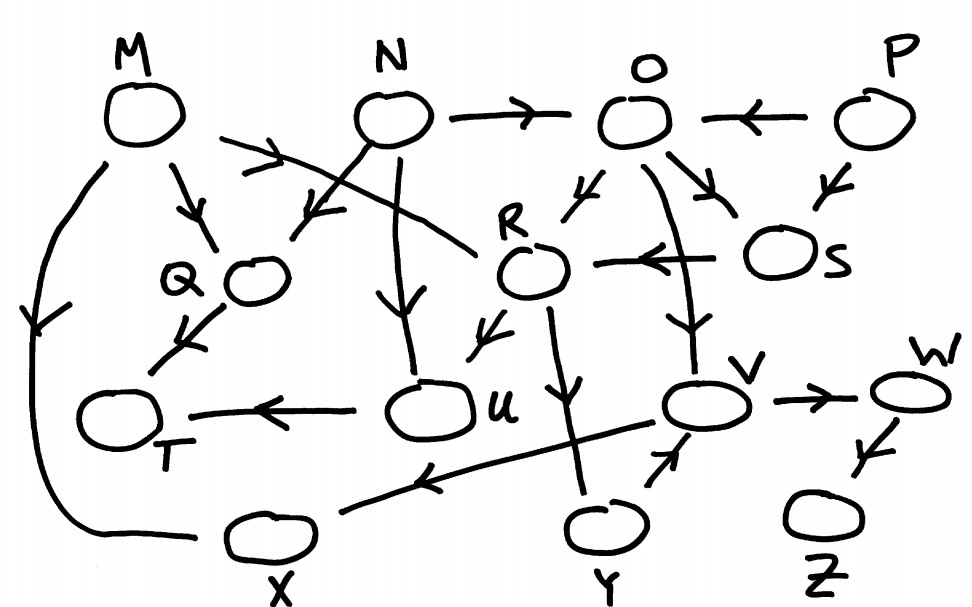
\includegraphics[width=90mm]{figureC.jpg}
\end{center}
    \textbf{TOP-SORT(G)}
    \begin{itemize}
        \item [1.] Call DFS(G) to compute finishing times f[v] for each vertex v.
        \item [2.] As each vertex finishes, insert it onto the front of a linked list.
        \item [3.] Return the linked list of vertices.
    \end{itemize}
    The first letter is M so we apply DFS starting from M.
    \begin{center}
        \begin{tabular}{|c | c | c |} 
        \hline
        v & s[v] & f[v] \\ [0.5ex] 
        \hline\hline
        M & 1 & 20 \\
        \hline
        \textcolor{red}{X} & 2 & 3 \\
        \hline
        Q & 4 & 7 \\
        \hline
        T & 5 & 6 \\
        \hline
        R & 8 & 19 \\
        \hline
        U & 9 & 10 \\
        \hline
        Y & 11 & 18 \\
        \hline
        V & 12 & 17 \\
        \hline
        W & 13 & 16 \\
        \hline
        Z & 14 & 15 \\ [1ex] 
        \hline
        \end{tabular}
    \end{center}
    Now N, O, P and S are still white so we do DFS-VISIT(N) (as N after M in alphabet):
    \begin{center}
        \begin{tabular}{|c | c | c |} 
        \hline
        v & s[v] & f[v] \\ [0.5ex] 
        \hline\hline
        N & 21 & \textcolor{red}{26} \\
        \hline
        O & 22 & 25 \\
        \hline
        S & 23 & 24 \\ [1ex] 
        \hline
        \end{tabular}
    \end{center}
    \\ Finally, we need to do P:
    \begin{center}
        \begin{tabular}{|c | c | c |} 
        \hline
        v & s[v] & f[v] \\ [0.5ex] 
        \hline\hline
        P & 27 & 28 \\ [1ex]
        \hline
        \end{tabular}
    \end{center}
    Now, the linked list of the reversed order of vertices according to their finishing times is: PNOSMRYVWZUQTX
    \\ Practically, as soon as a vertex finishes, we just add it to the head of a linked list.
    
\item \textbf{\textcolor{blue}{Let $G$ be a DAG with a specific designated vertex $v$. Uno and Dos (Spanish for One and Two) play the following game. A token is placed on $v$.  The players alternate moves, Uno playing first.  On each turn if the token is on $w$ the player moves the token to some vertex $u$ with $(w,u)$ an edge of the DAG. When a player has no move, he or she loses. Except for the first part below, we assume Uno and Dos play perfectly.}}
\begin{enumerate}
    \item \textbf{\textcolor{blue}{Argue that the game {\em must} end. Indeed, argue that if     $G$ has $n$ vertices then the game {\em cannot} take more than $n-1$ moves. (Key: Its a DAG!)}}
        \\ \textbf{DAG:} Directed acyclic graph (no loops)
        \\ Let G have n vertices. If the game went on for n moves, the chip would hit n+1 positions $v_0, v_1, ..., v_n$. Because there are only n vertices, it means some positions would be hit more than once. However, the graph is acyclic so this is not possible. Hence the game must end after n-1 moves.
    \item \textbf{\textcolor{blue}{Define {\tt VALUE[z]} to be the winner of the game (either Uno or Dos) where the token is initially placed at vertex $z$ and Uno plays first. (That is, {\tt VALUE[z]} being Uno means that the player who has the move will win, {\tt VALUE[z]} being Dos means that the player who has the move will lose.) When $z$ is a leaf node and Uno plays first, Uno has no move and so loses and therefore {\tt VALUE[z]} is Dos.  But what if $z$ is {\em not} a leaf node. Suppose the {\tt VALUE[w]} are known for all $w\in Adj[z]$. How do those values determine {\tt VALUE[z]}? (To give part of the answer: Suppose there is some $w\in Adj[z]$ with {\tt VALUE[w]} equal Dos. From $z$ Uno's winning strategy is to move to $w$.)}}
        \\ Suppose $\exists \ w \in Adj[z]$ with VALUE[w] = Dos.
        \\ Uno makes the move. As the roles are reversed and Dos moves first, Uno wins so VALUE[z] = Uno.
        \\ Otherwise, a position w is reached with VALUE[w] = Uno (whatever Uno does). Dos, who is making the first move, wins so VALUE[z] = Dos.
    \item \textbf{\textcolor{blue}{Using the above idea modify {\tt DFS-VIST[v]} to find who wins the original game.  In your modified algorithm there will be an extra function {\tt VALUE[w]} which is originally set to {\tt NIL} for all vertices $w$, representing that the winner of the game starting at $w$ has not yet been determined. When the unmodified {\tt DFS-VISIT[w]} would be finished add a couple of lines of pseudocode to give {\tt VALUE[w]}. Give an upper bound on the time of your algorithm.}}
        \\ Apply the following DFS-VISIT-CUSTOM[G, v]. \\
        \begin{algorithm}[H]
        \SetKwFunction{dfsc}{DFS-VISIT-CUSTOM}
        \Indm\dfsc{G, v}\\
        \Indp
            time = time + 1 \\
            d[u] = time \\
            color[u] = GRAY \\
            value[u] = Dos \\
            \For{each vertex v $\in$ G.Adj[u]}{
                \If{color[v] == WHITE}{
                    $\pi$[v] = u \\
                    DFS-VISIT-CUSTOM(G, v) \\
                }
                \If{value[v] == Dos}{
                    value[u] = Uno \\
                }
            }
            color[u] = BLACK \\
            time = time + 1 \\
            f[u] = time \\
            \caption{DFS-VISIT-CUSTOM[G, v] algorithm}
        \end{algorithm}
        This algorithm requires O(V+E), but could be smaller as the algorithm only reach a small of the graph.
    \end{enumerate}
\end{enumerate}

\end{document}